%%%%%%%%%%%%%%%%%%%%%%%%%%%%%%%%%%%%%%%%%%%%%%%%
% Template TCMN data sheet version 3
% 
% Alberto Sanchez asanchezrodelgo@ifc.org Dec 2015
%%%%%%%%%%%%%%%%%%%%%%%%%%%%%%%%%%%%%%%%%%%%%%%%
\documentclass{article}\usepackage[]{graphicx}\usepackage[]{color}
%% maxwidth is the original width if it is less than linewidth
%% otherwise use linewidth (to make sure the graphics do not exceed the margin)
\makeatletter
\def\maxwidth{ %
  \ifdim\Gin@nat@width>\linewidth
    \linewidth
  \else
    \Gin@nat@width
  \fi
}
\makeatother

\definecolor{fgcolor}{rgb}{0.345, 0.345, 0.345}
\newcommand{\hlnum}[1]{\textcolor[rgb]{0.686,0.059,0.569}{#1}}%
\newcommand{\hlstr}[1]{\textcolor[rgb]{0.192,0.494,0.8}{#1}}%
\newcommand{\hlcom}[1]{\textcolor[rgb]{0.678,0.584,0.686}{\textit{#1}}}%
\newcommand{\hlopt}[1]{\textcolor[rgb]{0,0,0}{#1}}%
\newcommand{\hlstd}[1]{\textcolor[rgb]{0.345,0.345,0.345}{#1}}%
\newcommand{\hlkwa}[1]{\textcolor[rgb]{0.161,0.373,0.58}{\textbf{#1}}}%
\newcommand{\hlkwb}[1]{\textcolor[rgb]{0.69,0.353,0.396}{#1}}%
\newcommand{\hlkwc}[1]{\textcolor[rgb]{0.333,0.667,0.333}{#1}}%
\newcommand{\hlkwd}[1]{\textcolor[rgb]{0.737,0.353,0.396}{\textbf{#1}}}%

\usepackage{framed}
\makeatletter
\newenvironment{kframe}{%
 \def\at@end@of@kframe{}%
 \ifinner\ifhmode%
  \def\at@end@of@kframe{\end{minipage}}%
  \begin{minipage}{\columnwidth}%
 \fi\fi%
 \def\FrameCommand##1{\hskip\@totalleftmargin \hskip-\fboxsep
 \colorbox{shadecolor}{##1}\hskip-\fboxsep
     % There is no \\@totalrightmargin, so:
     \hskip-\linewidth \hskip-\@totalleftmargin \hskip\columnwidth}%
 \MakeFramed {\advance\hsize-\width
   \@totalleftmargin\z@ \linewidth\hsize
   \@setminipage}}%
 {\par\unskip\endMakeFramed%
 \at@end@of@kframe}
\makeatother

\definecolor{shadecolor}{rgb}{.97, .97, .97}
\definecolor{messagecolor}{rgb}{0, 0, 0}
\definecolor{warningcolor}{rgb}{1, 0, 1}
\definecolor{errorcolor}{rgb}{1, 0, 0}
\newenvironment{knitrout}{}{} % an empty environment to be redefined in TeX

\usepackage{alltt}
%%%%%%%%%%%%%% package declaration %%%%%%%%%%%%%%%%%%%%%
\usepackage[top=0.3in, bottom=0.1in, left=0.5in, right=0.6in]{geometry}
\usepackage{graphicx} % to load images
\usepackage[export]{adjustbox} % add alignment to includegraphics
\usepackage[font=small]{caption}
\usepackage{xcolor} % color text
\usepackage{tabularx} % to adjust table width, etc. 
\usepackage{titlesec} % format titles and headers
\usepackage{sectsty} % format sections & subsections
\usepackage{booktabs} % For \toprule, \midrule and \bottomrule
\usepackage[colorlinks = true,
            linkcolor = blue,
            urlcolor  = blue,
            citecolor = blue,
            anchorcolor = blue]{hyperref} % to include hyperlinks in the doc
\sectionfont{\fontsize{16}{15}\selectfont\raggedright} % formats title newsletter (section) 
\subsectionfont{\fontsize{14}{12}\selectfont\raggedright} % formats title newsletter (section)
%%%%%%%%%%%%%%%%%%%%%%%%%%%%%%%%%%%%%%%%%%%%%%%%%%%%%%%%%%%%%%%%%%%%%%%%%%%%%%%%%%%
%
%%%%%%%%%%%%%%%%%%%%%%%%%%%%%%%%%%%%% BEGIN DOCUMENT %%%%%%%%%%%%%%%%%%%%%%%%%%%%%%
\IfFileExists{upquote.sty}{\usepackage{upquote}}{}
\begin{document}

%

%%%%%%%%%%%%%%%% PAGE 1 %%%%%%%%%%%%%%%%%%%
%World Bank logo and TCMN branding
\begin{figure}
  \vspace{-3ex} % move up this figure
  \hspace{-7ex} % move left this figure
  \includegraphics[width=5cm]{/Users/asanchez3/shinyTCMN/www/wb_logo_background.png}
\end{figure}
\begin{figure}
  \begin{minipage}[t]{0.99\textwidth} % top section
      \vspace{-30ex}
      \hspace{-2ex}
      \raggedright{\includegraphics[width=5.5cm,right]{/Users/asanchez3/shinyTCMN/www/TC_snapshots_data.png}}
  %  {\color{white!70!black}\noindent\makebox[\linewidth]{\rule{20cm}{0.3pt}}} % horiz line
  \end{minipage}
\end{figure}
%
%%%% Macro Indicators
\begin{minipage}[t]{0.99\textwidth} % top section
  \vspace{-1.5cm}
  \begin{minipage}[c]{0.36\textwidth} 
    \begin{minipage}[c]{0.28\textwidth} % flag
      \includegraphics[width=1.2cm,height=1.2cm]{/Users/asanchez3/shinyTCMN/www/IN.png}
    \end{minipage}
    \begin{minipage}[c]{0.70\textwidth} % Country name
      \section*{\color{blue!40!black}India}
    \end{minipage}
  \end{minipage}
  \begin{minipage}[c]{0.63\textwidth} % key macro table 
    % Table 1
    \centering
    \resizebox{\textwidth}{!}{
% latex table generated in R 3.2.2 by xtable 1.7-4 package
% Tue May 31 11:05:37 2016
{\LARGE
\begin{tabular}{>{\centering}p{1.5in}>{\centering}p{1.5in}>{\centering}p{1.5in}>{\centering}p{1.5in}>{\centering}p{1.5in}>{\centering}p{1.5in}>{\centering}p{1.5in}l}
  GDP (US\$ billions) (2017) & Population (millions) (2017) & Land area (sq. km) (2015) & Income per capita (current US\$) (2017) & Poverty rate (2011) \large{[1]} & Unemployment rate (2016) & Ease of Doing Business Rank (2016) &  \\ 
      2,841 &     1,343 & 2,973,190 &     2,116 &        21 &        NA &       130 &  \\ 
  \end{tabular}
}

    }
  \end{minipage}  
\end{minipage} % end top section

\begin{minipage}[b]{0.99\textwidth} % macro indicators main table
  %\vspace*{0.5cm}
  %\vspace{+3ex}
  \begin{minipage}[t]{0.99\textwidth}

    \begin{minipage}[c]{0.875\textwidth}
      \begin{flushleft}  
      {\color{white!30!blue} \textbf{\small Macro Indicators}}
      \end{flushleft} 
      \vspace*{-0.4cm}
      % Table 2
      \centering
      \resizebox{\textwidth}{!}{
% latex table generated in R 3.2.2 by xtable 1.7-4 package
% Tue May 31 11:05:38 2016
{\Large
\begin{tabular}{>{\raggedright}p{6in}r>{\raggedleft}p{0.8in}>{\raggedleft}p{0.8in}>{\raggedleft}p{0.8in}>{\raggedleft}p{0.8in}>{\raggedleft}p{0.8in}l}
  & Avg 2003-2012 & 2013 & 2014 & 2015 & 2016 & 2017 &  \\ 
  \hline
GDP growth (annual \%) &   7.3 &   6.9 &   7.3 &   7.5 &   7.8 &   7.9 &  \\ 
  Current account balance &  -1.3 &  -1.7 &  -1.3 &  -1.4 &  -1.7 &  -2.0 &  \\ 
  Fiscal balance (\% of GDP) &  -8.4 &  -7.3 &  -7.0 &  -6.4 &  -6.1 &  -5.7 &  \\ 
  Remittances, received (\% of GDP) \large{[1]} &   3.3 &   3.8 &   3.4 & --- & --- & --- &  \\ 
  General government gross debt \large{[3]} &  75.8 &  66.2 &  66.3 &  67.2 &  66.5 & --- &  \\ 
  Real Effective Exchange Rate (2010=100) &  98.8 &  89.1 &  94.7 & 103.0 & 105.7 & 108.9 &  \\ 
  Consumer Price Index, annual percent change &   6.8 &   9.9 &   6.0 &   5.0 &   4.0 &   4.0 &  \\ 
  \end{tabular}
}

      }
    \end{minipage}
    \begin{minipage}[c]{0.11\textwidth}
      \vspace*{+0.8cm}


{\centering 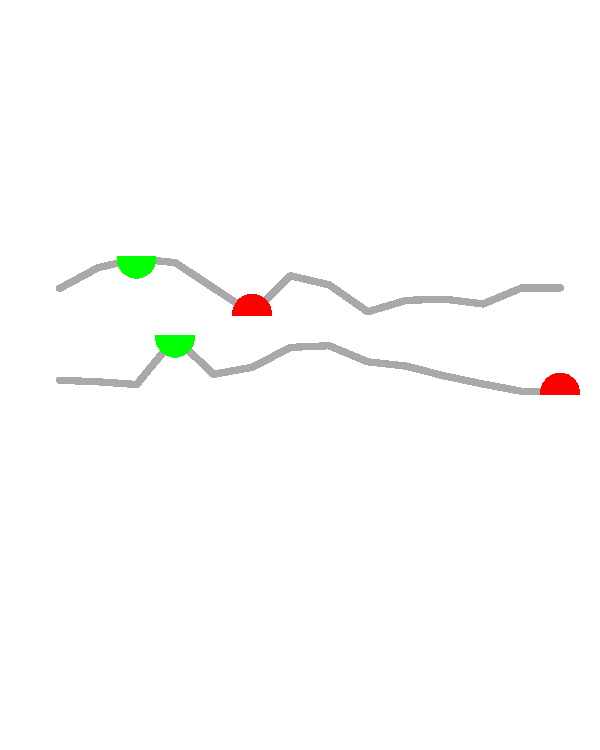
\includegraphics[width=\maxwidth]{figure/createSparklines_macro-1} 

}



      \vspace*{-0.5cm}
    \end{minipage}
    
    %\vspace*{-0.4cm}
    \begin{minipage}[c]{0.875\textwidth}
      \begin{flushleft}  
      {\color{white!30!blue} \textbf{\small Investment indicators}}
      \end{flushleft} 
      \vspace*{-0.4cm}
      % Table 2
      \centering
      \resizebox{\textwidth}{!}{
% latex table generated in R 3.2.2 by xtable 1.7-4 package
% Tue May 31 11:05:38 2016
{\Large
\begin{tabular}{>{\raggedright}p{6in}r>{\raggedleft}p{0.8in}>{\raggedleft}p{0.8in}>{\raggedleft}p{0.8in}>{\raggedleft}p{0.8in}>{\raggedleft}p{0.8in}l}
  & Avg 2003-2012 & 2013 & 2014 & 2015 & 2016 & 2017 &  \\ 
  \hline
Gross domestic investment (\% GDP) & 28.7 & 30.7 & 30.0 & 30.1 & 30.5 & 30.9 &  \\ 
  Gross domestic investment, of w: Private investment (\% GDP) \large{[1]} & 35.0 & 32.3 & 31.6 & --- & --- & --- &  \\ 
  Inward FDI (\% of GDP) \large{[2]} &  1.7 &  1.5 &  1.7 & --- & --- & --- &  \\ 
  Inward FDI, \% of private investment \large{[2]} &  5.3 &  4.9 &   NA & --- & --- & --- &  \\ 
  \end{tabular}
}

      }
    \end{minipage}
    \begin{minipage}[c]{0.11\textwidth}
      \vspace*{+0.8cm}


{\centering 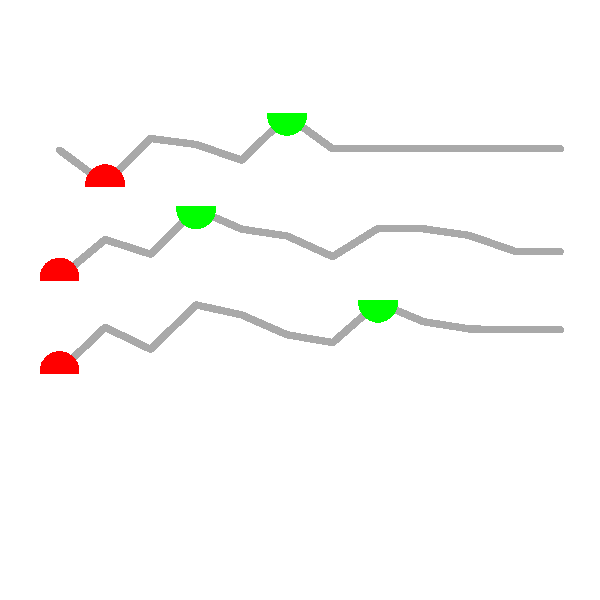
\includegraphics[width=\maxwidth]{figure/createSparklines_invest-1} 

}



      \vspace*{-0.5cm}
    \end{minipage}
    
    %\vspace*{-0.4cm}
    \begin{minipage}[c]{0.875\textwidth}
      \begin{flushleft}  
      {\color{white!30!blue} \textbf{\small Trade Indicators}}
      \end{flushleft} 
      \vspace*{-0.4cm}
      % Table 2
      \centering
      \resizebox{\textwidth}{!}{
% latex table generated in R 3.2.2 by xtable 1.7-4 package
% Tue May 31 11:05:38 2016
{\Large
\begin{tabular}{>{\raggedright}p{6in}r>{\raggedleft}p{0.8in}>{\raggedleft}p{0.8in}>{\raggedleft}p{0.8in}>{\raggedleft}p{0.8in}>{\raggedleft}p{0.8in}l}
  & Avg 2003-2012 & 2013 & 2014 & 2015 & 2016 & 2017 &  \\ 
  \hline
Total Trade in Goods and Services (\% of GDP, real terms) & 41.59 & 51.30 & 47.11 & 45.14 & 44.39 & 44.31 &  \\ 
  Trade balance (\% GDP, real terms) & -3.05 & -1.85 & -1.37 & -1.31 & -1.50 & -1.94 &  \\ 
  Exports, Goods and Services, annual percent change (real terms) & 13.86 &  7.28 & -0.76 &  3.00 &  5.50 &  6.60 &  \\ 
  Imports, Goods and Services, annual percent change (real terms) & 14.87 & -8.38 & -2.14 &  3.00 &  6.50 &  8.75 &  \\ 
  Total reserves in months of imports \large{[1]} &  8.95 &  6.03 &  6.61 & --- & --- & --- &  \\ 
  \end{tabular}
}

      }
    \end{minipage}
    \begin{minipage}[c]{0.11\textwidth}
      \vspace*{+0.8cm}


{\centering 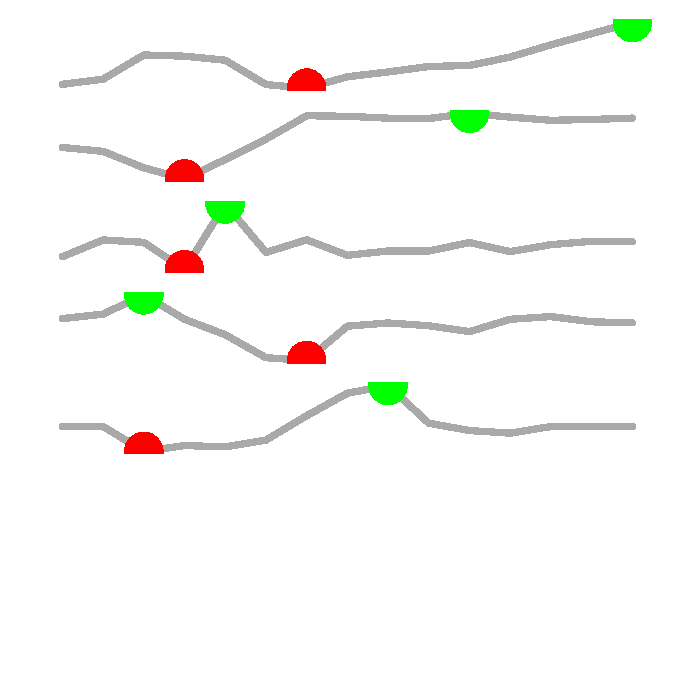
\includegraphics[width=\maxwidth]{figure/createSparklines_trade-1} 

}



      \vspace*{-0.4cm}
    \end{minipage}
  \\[3pt]
\raggedright{\footnotesize{\href{http://www.worldbank.org/en/topic/macroeconomics/overview}{Sources: MFM note}{,} \href{http://data.worldbank.org/data-catalog/world-development indicators}{[1] World Development Indicators (WDI)}{,} \href{http://unctadstat.unctad.org/wds/ReportFolders/reportFolders.aspx}{[2] UNCTADSTAT}{,} \href{https://www.imf.org/external/pubs/ft/weo/2015/02/weodata/index.aspx}{[3] World Economic Outlook (WEO)}}}
  \end{minipage} 
%\end{minipage}    
  \begin{minipage}[b]{\textwidth} % macro charts
  \vspace{+3ex}
    \begin{minipage}[c]{0.49\textwidth} % imports/exports 
    \center{\color{blue!50!black} \textbf{\small Goods Export and Import \\ volume growth, 2012-2015}}


{\centering 
\includegraphics[width=\maxwidth]{figure/ExpImp_HF-1} 

}



    \vspace*{-0.3cm}
    %\hspace*{0.5cm} 
    \raggedright{\footnotesize{\href{http://web.worldbank.org/WBSITE/EXTERNAL/EXTDEC/EXTDECPROSPECTS/0,,menuPK:476941~pagePK:51084723~piPK:51084722~theSitePK:476883,00.html}{Source: Development Prospects Group (DECPG)}}}
    \end{minipage}
    \begin{minipage}[c]{0.49\textwidth} % gdp value added
    \center{\color{blue!50!black} \textbf{\small Gross Value Added by \\ Economic Activity 2013 \footnotesize(\% GDP)}}


{\centering 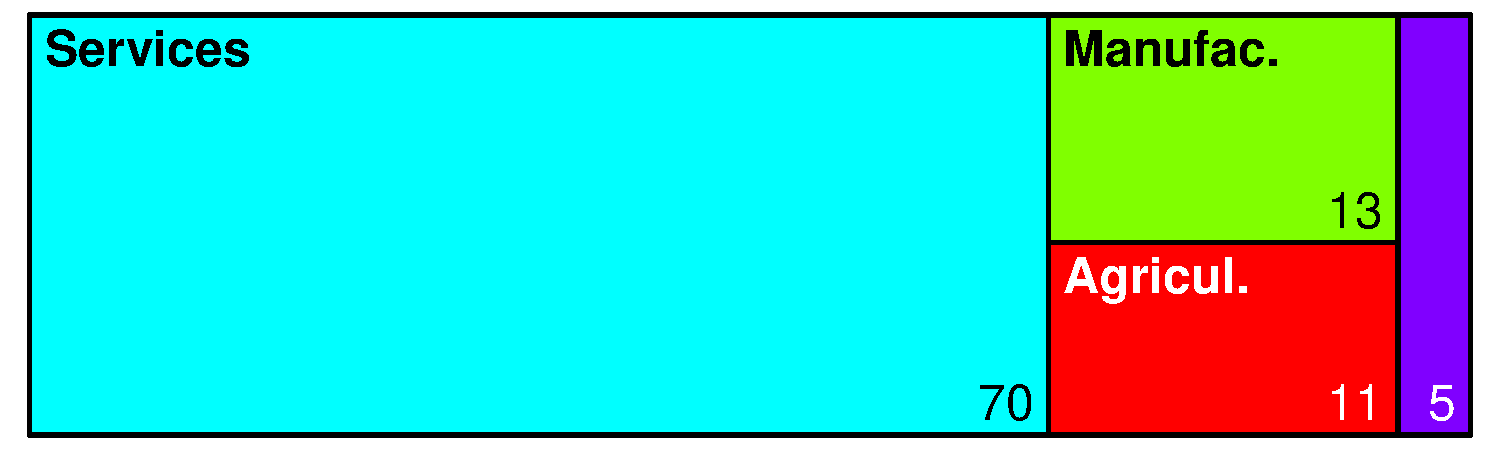
\includegraphics[width=\maxwidth]{figure/GVA_Treemap-1} 

}



   %\vspace*{-0.3cm}
   %\hspace*{0.5cm} 
   \raggedright{\footnotesize{\href{http://data.worldbank.org/data-catalog/world-development indicators}{Source: World Development Indicators (WDI)}}}
    \end{minipage}
  \end{minipage}  
\end{minipage}   
 
%%%% Exports Imports and DB
\begin{minipage}[b]{0.99\textwidth}
  \vspace{0.8cm}
   \begin{minipage}[c]{0.44\textwidth} 
    %\vspace*{-0.2cm}
    \begin{minipage}[t]{0.99\textwidth} 
      {\color{blue!50!black} \textbf{\small Top 5 Exports by \% of Total Value, 2015}}
      %\vspace{3ex}
      \\[6pt]
      \centering
      \resizebox{\textwidth}{!}{%


{\centering 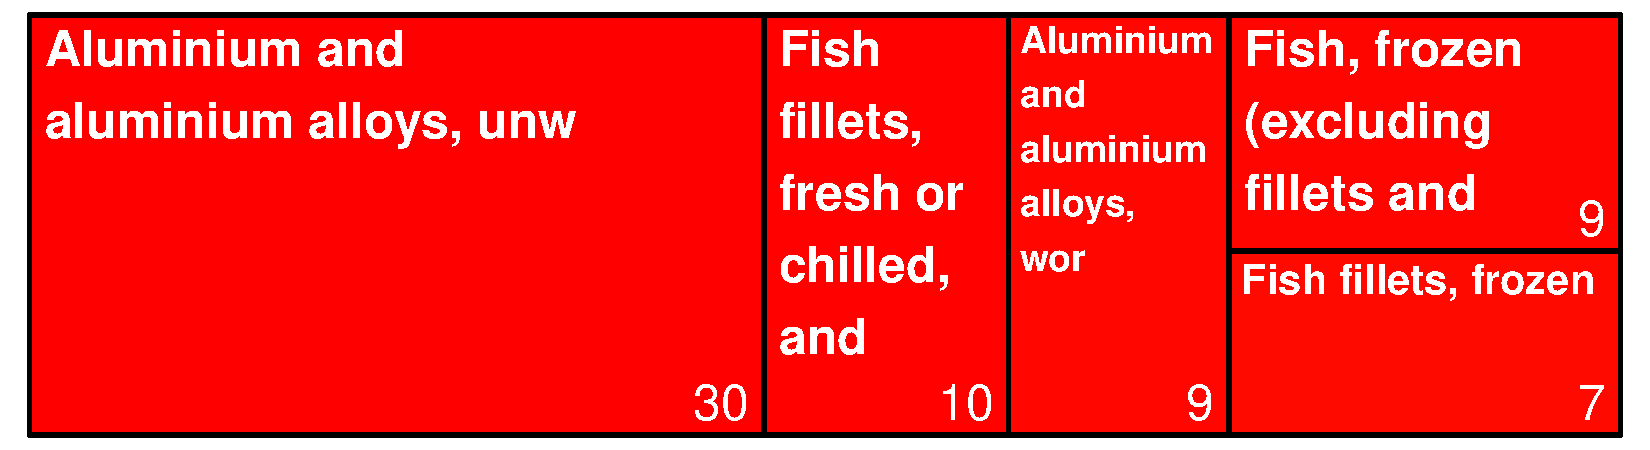
\includegraphics[width=\maxwidth]{figure/ImpExp_Treemap-2-1} 

}



      }
      \end{minipage}
      \\[14pt]
      \begin{minipage}[t]{0.99\textwidth} 
      {\color{blue!50!black} \textbf{\small Imports Categories by \% of Total Value, 2015}}
      \\[6pt]
      \centering
      \resizebox{\textwidth}{!}{%


{\centering 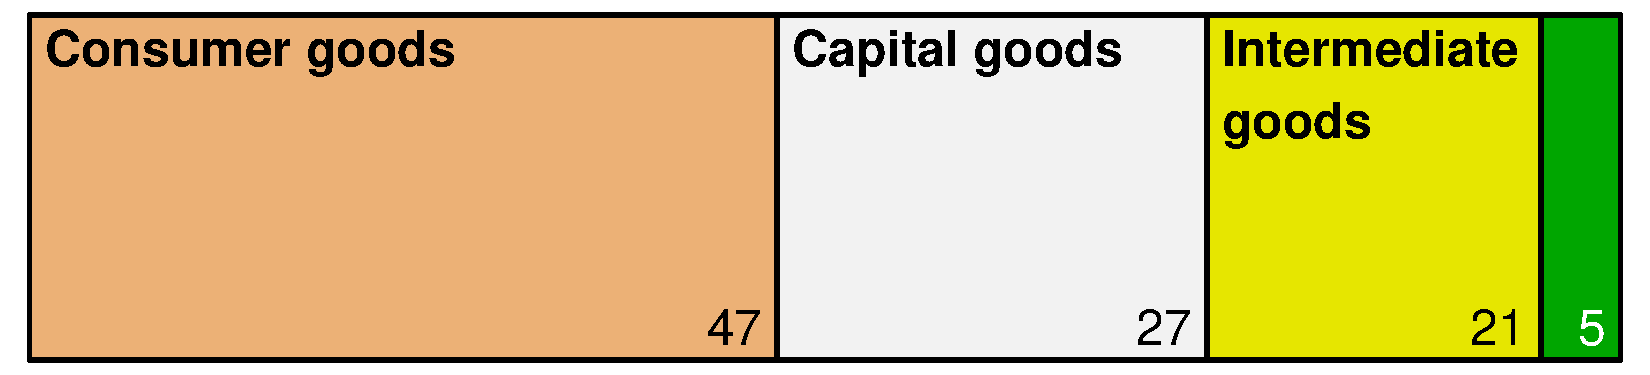
\includegraphics[width=\maxwidth]{figure/ImpExp_Treemap-1-1} 

}



      }
      \end{minipage}
      \\[10pt]
    %\hspace*{0.5cm}
    \footnotesize{\href{http://wits.worldbank.org}{Source: World Integrated Trade Solution (WITS)}} 
    \end{minipage}
    \begin{minipage}[c]{0.56\textwidth} % Doing Business table
    %\vspace*{-0.1cm}
    %\begin{flushleft}
      \center {\color{blue!50!black}\textbf{\small Doing Business 2015 \\ \footnotesize Distance to Frontier (DTF) and Rank}}
    %\end{flushleft}
    \\[18pt]
    \centering
      \resizebox{\textwidth}{!}{%
% latex table generated in R 3.2.2 by xtable 1.7-4 package
% Tue May 31 11:05:39 2016
{\large
\begin{tabular}{lrrr|rrrr}
  &  & DTF &  &  & Rank &  &  \\ 
  &  2015 &  2016 &  Change & 2015 & 2016 & Change &  \\ 
   \hline
\textbf{Ease of Doing Business} & \textbf{52.67} & \textbf{54.68} & \textbf{\color{green}{2.01}} & \textbf{134} & \textbf{130} & \textbf{\color{green}{4}} &  \\ 
  Dealing with Construction Permits & 32.47 & 32.47 & 0 & 184 & 183 & \color{green}{1} &  \\ 
  Enforcing Contracts & 32.41 & 32.41 & 0 & 178 & 178 & 0 &  \\ 
  Getting Credit & 65 & 65 & 0 & 36 & 42 & \color{red}{-6} &  \\ 
  Getting Electricity & 64.39 & 74.56 & \color{green}{10.17} & 99 & 70 & \color{green}{29} &  \\ 
  Paying Taxes & 56.14 & 56.14 & 0 & 156 & 157 & \color{red}{-1} &  \\ 
  Protecting Minority Investors & 73.33 & 73.33 & 0 & 8 & 8 & 0 &  \\ 
  Registering Property & 50.22 & 50.29 & \color{green}{0.07} & 138 & 138 & 0 &  \\ 
  Resolving Insolvency & 32.6 & 32.59 & \color{red}{-0.01} & 136 & 136 & 0 &  \\ 
  Starting a Business & 63.69 & 73.59 & \color{green}{9.9} & 164 & 155 & \color{green}{9} &  \\ 
  Trading Across Borders & 56.45 & 56.45 & 0 & 133 & 133 & 0 &  \\ 
  \end{tabular}
}

      }
    \\[15pt]
     %\hspace*{0.5cm} 
     \raggedright{\footnotesize{\href{http://www.doingbusiness.org/data}{Source: Doing Busines Report 2015}}}
    \end{minipage}
\end{minipage}

% \vspace{+3ex}
% {\color{blue!50!white}\noindent\makebox[\linewidth]{\rule{18cm}{0.3pt}}} % horiz line
% \begin{minipage}[c]{0.99\textwidth}
%   \hspace*{-0.4cm}\raggedleft{\color{white!40!black} \footnotesize TRADE AND COMPETITIVENESS MONITORING NOTE - UPDATED} 
%   %month year}
% \end{minipage}

\newpage
%%%%%%%%%%%%%%%% PAGE 2 %%%%%%%%%%%%%%%%%%%

\begin{minipage}[t]{0.99\textwidth}
  \vspace{0.5cm}
  \begin{minipage}[c]{0.48\textwidth} % WEF Radar
    \center{\color{blue!50!black} \textbf{WEF Competitiveness Indicators \\ \footnotesize(Scale 1-7, 7=best)}}
    \vspace*{-0.6cm}


{\centering 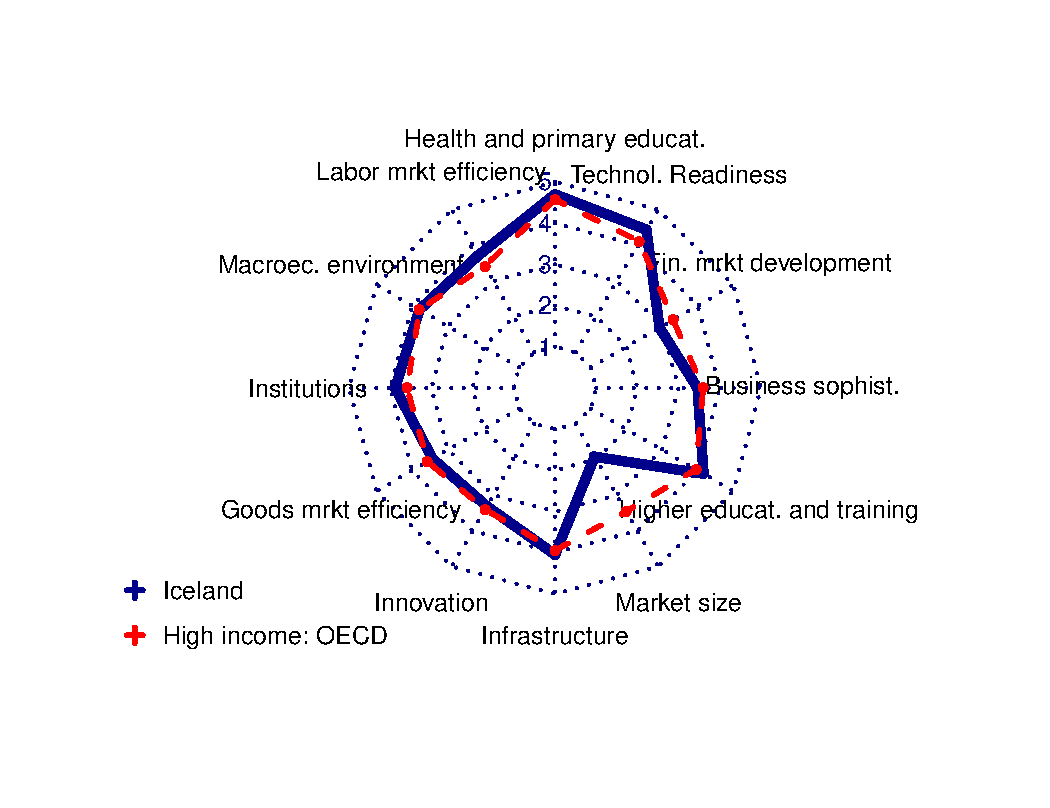
\includegraphics[width=\maxwidth]{figure/WEFradar-1} 

}



    \vspace*{-0.6cm} 
    \hspace*{0.3cm} \raggedright\footnotesize{\href{http://www.weforum.org/global-competitiveness-report-2015-2016}{Source: WEF Global Competitiveness Report 2015}}
  \end{minipage}
  \begin{minipage}[c]{0.50\textwidth} % LPI chart
  %\vspace*{0.5cm}
  \center {\color{blue!50!black} \textbf{Logistics Performance Index \\ \footnotesize(Scale 1-5, 5=best)}}
    \vspace*{0.4cm}


{\centering 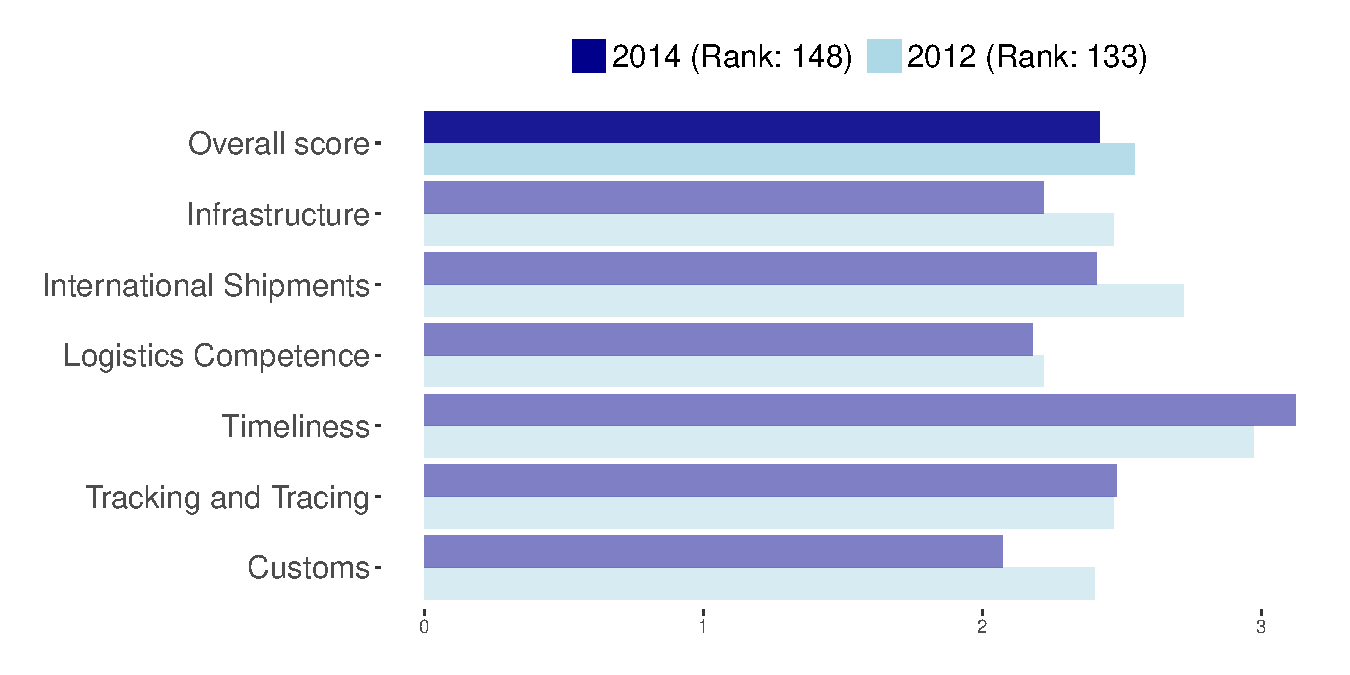
\includegraphics[width=\maxwidth]{figure/LPIindicators-1} 

}



  %\hspace*{0.5cm} 
  \raggedright\footnotesize{\href{http://lpi.worldbank.org}{Source: Logistics Performance Index (World Bank)}}
  \end{minipage}
\end{minipage}  

\begin{minipage}[b]{0.99\textwidth}
  \begin{minipage}[c]{0.50\textwidth} % WGI chart
    \vspace*{0.8cm}
    \center {\color{blue!50!black} \textbf{World Governance indicators \\ \footnotesize(Std. score, High=best)}}
    \vspace*{0.3cm}


{\centering 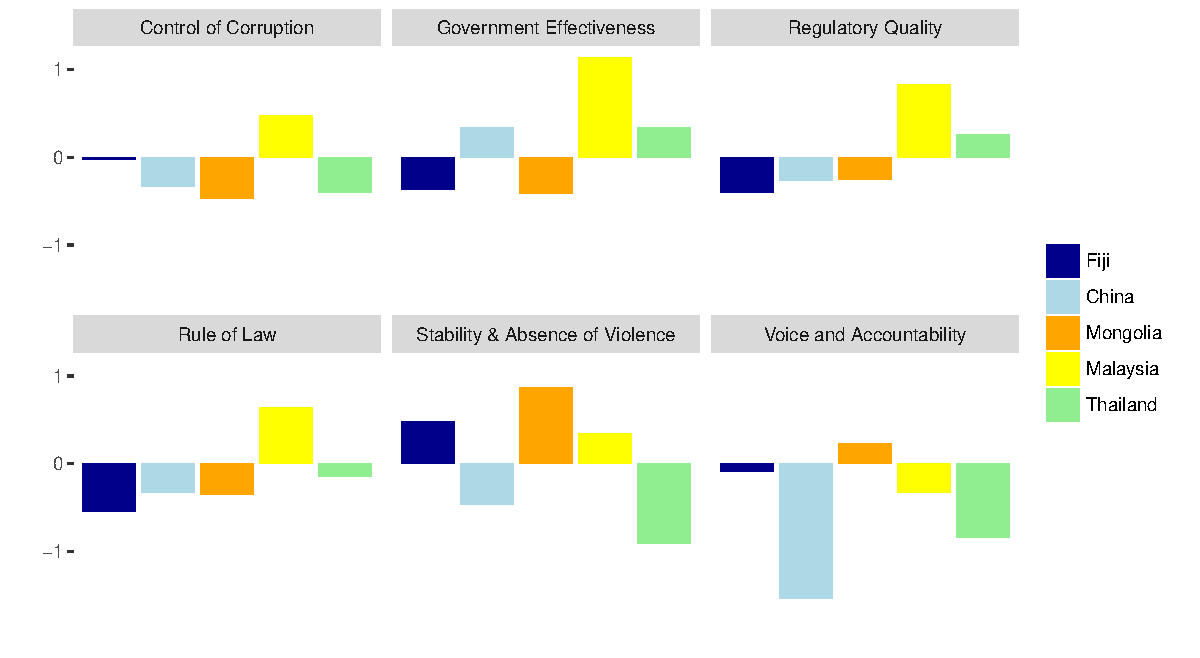
\includegraphics[width=\maxwidth]{figure/WGIindicators-1} 

}



    \vspace*{-0.6cm} 
    \hspace*{0.3cm} \raggedright\footnotesize{\href{http://data.worldbank.org/data-catalog/worldwide-governance-indicators}{Source: Worldwide Governance Indicators}}
  \end{minipage}
  \begin{minipage}[c]{0.48\textwidth} % Trade Policy table
    \vspace*{0.4cm}
  %\begin{flushleft}
    {\color{blue!50!black} \textbf{Trade Policy}}
  %\end{flushleft} 
  %\vspace*{0.2cm}
    \\[20pt]
    \centering
    \resizebox{\textwidth}{!}{%
% latex table generated in R 3.2.2 by xtable 1.7-4 package
% Tue May 31 11:05:40 2016
{\Large
\begin{tabular}{lrrr}
  & 2010 & 2014 &  \\ 
  \hline
Applied Tariff (Incl. Prefers. and Trade-Weighted) & 8.9 & --- &  \\ 
  Binding (\%) & 74.5 & --- &  \\ 
  Dispersion (Standard Deviation) & 15.3 & --- &  \\ 
  Import duties collected (\%, 2011-2013) \large{[1]} & --- & 5.8 &  \\ 
  MFN Tariff (Agriculture) & 31.4 & --- &  \\ 
  MFN Tariff (Non-Agriculture) & 9 & --- &  \\ 
  MFN Tariff (Simple Average) & 12.5 & --- &  \\ 
  Services sectors with GATS commitments \large{[1]} & --- & 37 &  \\ 
  \end{tabular}
}

    }
    \\[20pt]
    %\hspace*{0.5cm} 
    \raggedright{\footnotesize{\href{http://wits.worldbank.org}{Sources: WITS}{, }\href{http://stat.wto.org/CountryProfile/WSDBCountryPFHome.aspx?Language=E}{[1] WTO Trade Profiles}}}
  \end{minipage}
\end{minipage}

\vspace{+8ex}
%\hspace*{0.2cm}\subsection*{\color{white!50!black}Private Sector's Views}
\hspace*{0.1cm} \raggedright{\color{white!50!black}\Large Private Sector View}

\vspace*{-0.2cm}
{\color{white!30!black}\noindent\makebox[\linewidth]{\rule{18cm}{0.2pt}}} % horiz line

\begin{minipage}[b]{0.99\textwidth}
\vspace*{+0.6cm}
  \begin{minipage}[c]{0.02\textwidth}
  \hspace*{+0.1cm}
  \end{minipage}
  \begin{minipage}[c]{0.97\textwidth} 
    \begin{flushleft}  
      {\color{blue!50!black} \textbf{Enterprise Survey 2014}}
    \end{flushleft}  
    \vspace*{-0.4cm}
    \centering
    \resizebox{\textwidth}{!}{%
% latex table generated in R 3.2.2 by xtable 1.7-4 package
% Tue May 31 11:05:40 2016
{\Large
\begin{tabular}{lrrrl}
  & South Asia & India & All Countries &  \\ 
  \hline
Number of electrical outages in a typical month & 25.40 & 13.80 & 6.30 &  \\ 
  Percent of firms with a bank loan/line of credit & 27.00 & 21.30 & 35.20 &  \\ 
  Proportion of investments financed by banks (\%) & 14.40 & 18.10 & 14.60 &  \\ 
  Proportion of investments financed internally (\%) & 73.90 & 71.80 & 71.20 &  \\ 
  Senior management time spent dealing with the requirements of government regulation (\%) & 7.20 & 1.90 & 10.00 &  \\ 
  \end{tabular}
}

    }
    \\[8pt]
    %\hspace*{0.3cm} 
    \raggedright{\footnotesize{\href{https://www.enterprisesurveys.org/data}{Source: Enterprise Survey 2014}}}
  \end{minipage} 

  \begin{minipage}[b]{0.99\textwidth} 
    \vspace{+4ex}
    \begin{minipage}[c]{0.49\textwidth} % top 5 constraints ES
      \center{\color{blue!50!black} \textbf{Top 5 constraints according to ES 2014 \\ \footnotesize(\% respondants)}}


{\centering 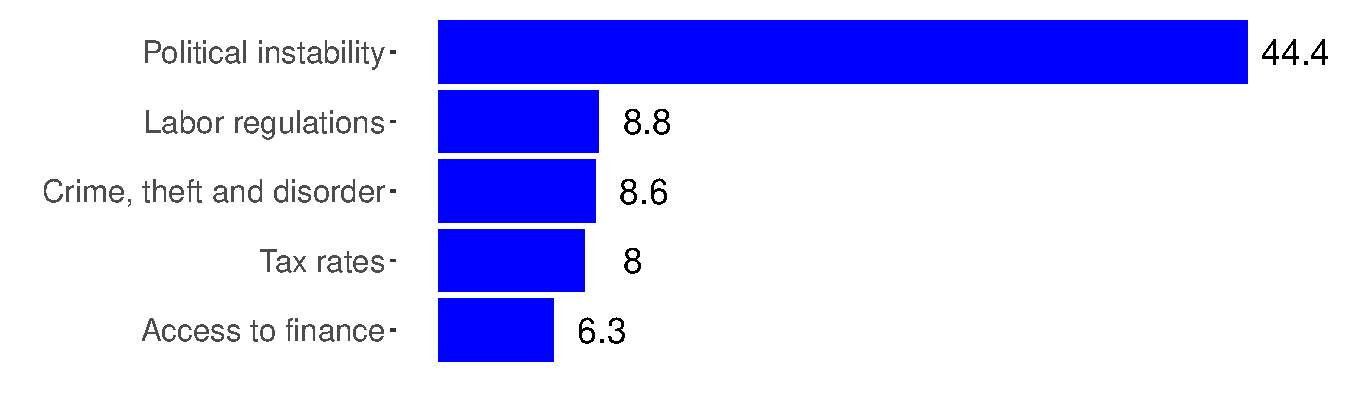
\includegraphics[width=\maxwidth]{figure/top5constraintsES-1} 

}



      %\vspace*{-0.7cm}
      \hspace*{0.3cm} \raggedright\footnotesize{\href{https://www.enterprisesurveys.org/data}{Source: Enterprise Survey 2014}}
    \end{minipage}
    \begin{minipage}[c]{0.49\textwidth} % top 5 constraints WEF
      \center{\color{blue!50!black} \textbf{Top 5 constraints according to WEF 2015 survey \\ \footnotesize(\% respondants among 88 executives)}}


{\centering 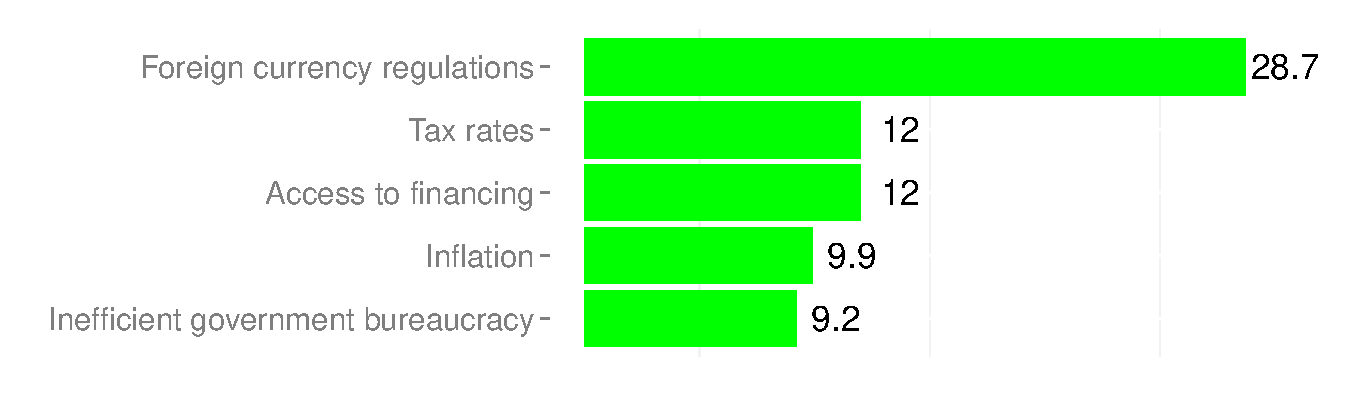
\includegraphics[width=\maxwidth]{figure/top5constraintsWEF-1} 

}



    %\vspace*{-0.7cm}
    \hspace*{0.3cm} \raggedright\footnotesize{\href{http://www.weforum.org/reports/global-competitiveness-report-2015-2016}{Source: WEF Global Competitiveness Report 2015}}
    \end{minipage}
  \end{minipage}
\end{minipage}

% \vspace{+8ex}
% {\color{blue!50!white}\noindent\makebox[\linewidth]{\rule{18cm}{0.3pt}}} % horiz line

% \vspace{+2ex}
% \begin{minipage}[c]{0.33\textwidth}
%   \hspace*{+0.3cm} \includegraphics[width=4cm,left]{/Users/asanchez3/shinyTCMN/www/wb_logo.jpg}
%   %\hspace*{+0.3cm} \includegraphics[width=4cm,left]{/Users/asanchez3/shinyTCMN/www/wb_logo.png}
% \end{minipage}
% \begin{minipage}[c]{0.65\textwidth}
%   \vspace*{-0.4cm}
%   \raggedleft{\color{white!40!black} \footnotesize TRADE AND COMPETITIVENESS MONITORING NOTE - UPDATED} 
%   %month year}
% \end{minipage}

%%%%%%%%%%%%%%%%%%%%%%%%%%%%%%%%%%%
%%%%%% Operations section %%%%%%%%%
%%%%%%%%%%%%%%%%%%%%%%%%%%%%%%%%%%%
\newpage
%%%%%%%%%%%%%%%% PAGE 3 %%%%%%%%%%%%%%%%%%%

%World Bank logo and TCMN branding
\begin{figure}
  \vspace{-3ex} % move up this figure
  \hspace{-7ex} % move left this figure
  \includegraphics[width=5cm]{/Users/asanchez3/shinyTCMN/www/wb_logo_background.png}
\end{figure}
\begin{figure}
  \begin{minipage}[t]{0.99\textwidth} % top section
      \vspace{-30ex}
      \hspace{-2ex}
      \raggedright{\includegraphics[width=5.5cm,right]{/Users/asanchez3/shinyTCMN/www/TC_snapshots_operations.png}}
  \end{minipage}
\end{figure}
%
%%%% Macro Indicators
\begin{minipage}[t]{0.99\textwidth} % top section
  \vspace{-1.5cm}
  \begin{minipage}[c]{0.36\textwidth} 
    \begin{minipage}[c]{0.28\textwidth} % flag
      \includegraphics[width=1.2cm,height=1.2cm]{/Users/asanchez3/shinyTCMN/www/IN.png}
    \end{minipage}
    \begin{minipage}[c]{0.70\textwidth} % Country name
      \section*{\color{blue!40!black}India}
    \end{minipage}
  \end{minipage}
  \begin{minipage}[c]{0.63\textwidth}
  %  \begin{flushleft}  
  %    \center{\color{blue!20!black} \textbf{\Large T\&C Product Line Operations Board Approved On or After FY14}}
  %  \end{flushleft} 
  \end{minipage}  
\end{minipage} % end top section

%\begin{minipage}[b]{0.99\textwidth} % main body
  \raggedright{\color{white!30!blue} \textbf{\Large SCD/CPF}}
    \begin{minipage}[c]{0.99\textwidth}  
      \vspace*{0.2cm}
      \raggedright{\color{white!30!blue} \textbf{\large Most Recent}}
      \vspace*{0.3cm}
      
% latex table generated in R 3.2.2 by xtable 1.7-4 package
% Tue May 31 11:05:40 2016
\scalebox{0.85}{
\begin{tabular}{>{\raggedright}p{5in}ll}
 Product & Document Date &  \\ 
  \hline
Performance and learning review of the country partnership strategy for India for the period FY2013 - 17 & 2015-10-21 &  \\ 
  \end{tabular}
}

      \vspace*{0.5cm}
    \end{minipage}
    
    \begin{minipage}[c]{0.99\textwidth} % imports/exports
      \vspace*{0.2cm}
      \raggedright{\color{white!30!blue} \textbf{\large Planned}}
      \vspace*{0.3cm}
      
% latex table generated in R 3.2.2 by xtable 1.7-4 package
% Tue May 31 11:05:40 2016
\scalebox{0.85}{
\begin{tabular}{>{\raggedright}p{5in}lll}
 Product & Concept Review Date & Board Date &  \\ 
  \hline
None &  &  &  \\ 
  \end{tabular}
}

      \vspace*{0.5cm}
    \end{minipage}
%\end{minipage}
  
\vspace*{0.5cm}
\raggedright{\color{white!30!blue} \textbf{\Large WB Lending Pipeline}}
\begin{minipage}[b]{0.99\textwidth} % overview tables
  \begin{minipage}[c]{0.99\textwidth}  
    \vspace*{0.5cm}
% latex table generated in R 3.2.2 by xtable 1.7-4 package
% Tue May 31 11:05:40 2016
{\scriptsize
\scalebox{0.85}{
\begin{tabular}{l>{\raggedright}p{1in}>{\raggedright}p{1in}>{\raggedright}p{0.5in}>{\raggedright}p{0.5in}>{\raggedright}p{0.5in}>{\raggedright}p{0.6in}>{\raggedright}p{0.5in}>{\raggedright}p{0.5in}>{\raggedleft}p{0.5in}>{\raggedleft}p{0.5in}l}
 Project ID & Project Name & Team Leader & Approval Date & Lending Inst. Type & Begin Appraisal & Commitment (US\$M) & Latest Sort Overall Risk Rating & FY Expenses (US\$K) & Cum Expenses (US\$K) & FY Prob &  \\ 
  \hline
P156241 & Innovate in India (I3) & Bharatha Manju S. Haththotuwa & 2017-07-27 & IPF & 2017-05-08 & 125 & --- & 13 & 13 & D &  \\ 
  \end{tabular}
}
}

    \vspace*{0.5cm}
  \end{minipage}
    
  \raggedright{\color{white!30!blue} \textbf{\Large WB Portfolio}}
  \begin{minipage}[c]{0.99\textwidth} % imports/exports
    \vspace*{0.2cm}
    \raggedright{\color{white!30!blue} \textbf{\large Active}}
    \vspace*{0.3cm}
      
% latex table generated in R 3.2.2 by xtable 1.7-4 package
% Tue May 31 11:05:41 2016
{\scriptsize
\scalebox{0.85}{
\begin{tabular}{l>{\raggedright}p{1in}>{\raggedright}p{1in}>{\raggedright}p{0.5in}>{\raggedright}p{0.5in}>{\raggedright}p{0.5in}>{\raggedleft}p{0.5in}>{\raggedleft}p{0.5in}>{\raggedright}p{0.4in}>{\raggedright}p{0.4in}>{\raggedright}p{0.4in}>{\raggedleft}p{0.4in}l}
 Project ID & Project Name & Team Leader & Approval Date & Lending Inst. Type & Closing Date & Commitment (US\$M) & Undisbursed Balance (US\$M) & Project Rating DO & Project Rating IP & Overall Risk & Months in Problem Status &  \\ 
  \hline
P145502 & TECHNOLOGY CENTER SYSTEMS PROJECT & Michael Olavi Engman & 2014-04-25 & IPF & 2020-06-30 & 200 & 196 & S & MS & M &  0 &  \\ 
  P048284 & STRENG.PROC.CAPACITY & Natarajan Raman & 1995-12-21 & --- & --- &   0 &  --- & --- & --- & --- & --- &  \\ 
  \end{tabular}
}
}

    \vspace*{0.5cm}
  \end{minipage}
     
  \begin{minipage}[c]{0.99\textwidth} % imports/exports 
    \raggedright{\color{white!30!blue} \textbf{\large Closed}}
    \vspace*{0.5cm}
      
% latex table generated in R 3.2.2 by xtable 1.7-4 package
% Tue May 31 11:05:41 2016
{\footnotesize
\scalebox{0.85}{
\begin{tabular}{l>{\raggedright}p{1.5in}>{\raggedright}p{1in}>{\raggedright}p{0.5in}>{\raggedright}p{0.5in}>{\raggedright}p{0.5in}>{\raggedleft}p{0.6in}>{\raggedright}p{0.5in}>{\raggedright}p{0.5in}>{\raggedright}p{0.5in}l}
 Project ID & Project Name & Team Leader & Approval Date & Lending Inst. Type & Closing Date & Commitment (US\$M) & Project Rating DO & Project Rating IP & IEG Outcome Rating &  \\ 
  \hline
None &  &  &  &  &  &  &  &  &  &  \\ 
  \end{tabular}
}
}

    \vspace*{0.5cm}
  \end{minipage}
     
\end{minipage}
 
 \newpage
%%%%%%%%%%%%%%%% PAGE 2 %%%%%%%%%%%%%%%%%%%
\begin{minipage}[t]{0.99\textwidth}
  \raggedright{\color{white!30!blue} \textbf{\Large WB ASA}}

  \begin{minipage}[b]{0.99\textwidth}
    \vspace*{0.2cm}
    \raggedright{\color{white!30!blue} \textbf{\large Active}}
    \vspace*{0.3cm}
  
% latex table generated in R 3.2.2 by xtable 1.7-4 package
% Tue May 31 11:05:41 2016
{\scriptsize
\scalebox{0.85}{
\begin{tabular}{l>{\raggedright}p{1in}>{\raggedright}p{1in}>{\raggedright}p{0.6in}>{\raggedright}p{0.6in}>{\raggedright}p{0.4in}>{\raggedright}p{0.4in}>{\raggedleft}p{0.6in}>{\raggedleft}p{0.6in}>{\raggedleft}p{0.6in}>{\raggedleft}p{0.6in}l}
 Task ID & Task Name & Team Leader & Concept Approval Date & Output Approval Date & Product Line & RAS (Y/N) & Current Expenditure BB (US\$K) & Current Expenditure Total (US\$K) & Lifetime Expenditure BB (US\$K) & Lifetime Expenditure Total (US\$K) &  \\ 
  \hline
P158432 & Support to DIPP on Startup India & Shihab Ansari Azhar & --- & 2017-12-31 & EW & N &   0 &  23 &   0 &  23 &  \\ 
  P154640 & India Ease of Doing Business - Track I & M. Masrur Reaz & --- & 2017-06-30 & TA & N &  --- &   0 &  --- &   0 &  \\ 
  P155802 & India Economic Integration Cluster & Juan Sebastian Saez & 2015-06-02 & 2017-06-30 & PA & N & 172 & 172 & 213 & 213 &  \\ 
  P158873 & India investment climate reforms & Shihab Ansari Azhar & --- & 2017-06-30 & TA & N &  --- &   0 &  --- &   0 &  \\ 
  P154653 & India Ease of Doing Business & M. Masrur Reaz & 2015-04-15 & 2017-06-23 & PA & N & 298 & 298 & 496 & 496 &  \\ 
  P159965 & Domestic Migration & Gaurav Nayyar & --- & 2016-12-31 & EW & N &  --- &   0 &  --- &   0 &  \\ 
  P159966 & Integration and Price Transmission & Gonzalo J. Varela & --- & 2016-12-31 & EW & N &  --- &   0 &  --- &   0 &  \\ 
  \end{tabular}
}
}

     \vspace*{0.2cm}
  \end{minipage}

  \begin{minipage}[b]{0.99\textwidth}
    \vspace*{0.2cm}
    \raggedright{\color{white!30!blue} \textbf{\large Closed}}
    \vspace*{0.3cm}
       
% latex table generated in R 3.2.2 by xtable 1.7-4 package
% Tue May 31 11:05:41 2016
{\scriptsize
\scalebox{0.85}{
\begin{tabular}{l>{\raggedright}p{1in}>{\raggedright}p{1in}>{\raggedright}p{0.6in}>{\raggedright}p{0.6in}>{\raggedright}p{0.4in}>{\raggedright}p{0.4in}>{\raggedleft}p{0.6in}>{\raggedleft}p{0.6in}>{\raggedleft}p{0.6in}>{\raggedleft}p{0.6in}l}
 Task ID & Task Name & Team Leader & Concept Approval Date & Output Approval Date & Product Line & RAS (Y/N) & Current Expenditure BB (US\$K) & Current Expenditure Total (US\$K) & Lifetime Expenditure BB (US\$K) & Lifetime Expenditure Total (US\$K) &  \\ 
  \hline
P149483 & Competitive Cities in India & Bertine Kamphuis & --- & 2016-03-22 & EW & N &  0 &  0 &  48 &    48 &  \\ 
  P132991 & Manufacturing Plan Implementation 2 & Bertine Kamphuis & 2012-12-06 & 2015-06-25 & TA & N & -1 & -1 & 457 & 1,049 &  \\ 
  P131209 & India manufacturing plan implementation & Luke Simon Jordan & --- & 2012-08-21 & TA & N & --- &  0 &  36 &    36 &  \\ 
  P120716 & PPIAF: INDIA: Capacity Bldg. for PPPs & Bhavna Bhatia & --- & 2010-04-30 & PT & N & --- &  0 &  --- &     0 &  \\ 
  P108043 & India:  HIV/AIDS, Stigma, and Inclusive & Gjorgjija Petkoski & 2007-07-20 & 2009-06-30 & TE & N & --- &  0 &  62 &   109 &  \\ 
  P090899 & Trade PNs III & Deepak K. Mishra & --- & 2006-06-30 & EW & N & --- &  0 & 128 &   128 &  \\ 
  P098785 & Dialogue on trade with Indian students & Carsten Fink & --- & 2005-10-12 & TE & N & --- &  0 &  --- &     0 &  \\ 
  P077091 & India Trade Policy & Deepak K. Mishra & --- & 2004-01-15 & EW & N & --- &  0 & 237 &   237 &  \\ 
  \end{tabular}
}
}

    \vspace*{0.5cm}
  \end{minipage}

  \raggedright{\color{white!30!blue} \textbf{\Large IFC ASA}}
  \begin{minipage}[b]{0.99\textwidth}
    \vspace*{0.2cm}
    \raggedright{\color{white!30!blue} \textbf{\large Active}}
    \vspace*{0.3cm}
  
% latex table generated in R 3.2.2 by xtable 1.7-4 package
% Tue May 31 11:05:41 2016
{\scriptsize
\scalebox{0.85}{
\begin{tabular}{l>{\raggedright}p{1.6in}>{\raggedright}p{1.5in}>{\raggedright}p{0.7in}>{\raggedright}p{0.7in}>{\raggedleft}p{0.7in}>{\raggedleft}p{0.7in}>{\raggedleft}p{0.7in}l}
 Project ID & Project Name & Team Leader & IP Approval Date & Expected End Date & Approval Value (in US\$K) & Total Expenditures (in US\$K) & Current FY Expenditure (in US\$K) &  \\ 
  \hline
600751 & India Ease of Doing Business & Azhar, Shihab Ansari & 2016-02-19 & 2018-02-28 & 2,743 &   429 & 340 &  \\ 
  600084 & Green Buildings in India & Purkayastha, Dhruba & 2015-04-17 & 2018-12-31 & 4,780 &   735 & 275 &  \\ 
  589787 & Odisha Inclusive Growth Partnership & Chodavarapu, Soujanya Krishna & 2013-02-20 & 2016-12-31 & 2,706 & 2,134 & 357 &  \\ 
  580727 & Buddhist Circuit Tourism: Facilitating Growth Corridors in UP and Bihar & Sharma, Monika & 2012-04-11 & 2017-06-30 & 3,797 & 1,796 &  93 &  \\ 
  601300 & India Automotive Competitiveness Project & Purkayastha, Dhruba & --- & --- &     0 &     0 &   0 &  \\ 
  \end{tabular}
}
}

    \vspace*{0.2cm}
  \end{minipage}

  \raggedright{\color{white!30!blue} \textbf{\large Pipeline}}
  \vspace*{0.3cm}
  
% latex table generated in R 3.2.2 by xtable 1.7-4 package
% Tue May 31 11:05:41 2016
{\footnotesize
\scalebox{0.85}{
\begin{tabular}{l>{\raggedright}p{1.6in}>{\raggedright}p{1.5in}>{\raggedright}p{0.7in}>{\raggedright}p{0.7in}>{\raggedleft}p{0.7in}>{\raggedleft}p{0.7in}>{\raggedleft}p{0.7in}l}
 Project ID & Project Name & Team Leader & IP Approval Date & Expected End Date & Approval Value (in US\$K) & Total Expenditures (in US\$K) & Current FY Expenditure (in US\$K) &  \\ 
  \hline
None &  &  &  &  &  &  &  &  \\ 
  \end{tabular}
}
}

  \vspace*{0.2cm}
\end{minipage}

\begin{minipage}[b]{0.99\textwidth}
  \raggedright{\color{white!30!blue} \textbf{\large Closed}}
  \vspace*{0.3cm}
  
% latex table generated in R 3.2.2 by xtable 1.7-4 package
% Tue May 31 11:05:41 2016
{\scriptsize
\scalebox{0.85}{
\begin{tabular}{l>{\raggedright}p{1.6in}>{\raggedright}p{1.5in}>{\raggedright}p{0.7in}>{\raggedright}p{0.7in}>{\raggedleft}p{0.7in}>{\raggedleft}p{0.7in}>{\raggedleft}p{0.7in}l}
 Project ID & Project Name & Team Leader & IP Approval Date & Expected End Date & Approval Value (in US\$K) & Total Expenditures (in US\$K) & Current FY Expenditure (in US\$K) &  \\ 
  \hline
580007 & Bihar IC Tax Simplification Program & Awasthi, Rajul & 2010-09-28 & 2013-06-30 &   783 &   601 & 0 &  \\ 
  568887 & India Rajasthan Investment Climate Reform  & Purkayastha, Dhruba & 2010-01-15 & 2014-09-30 & 3,370 & 3,116 & 0 &  \\ 
  568031 & BIHAR Investment Climate Reform Phase II & Oberai, Rina & 2009-01-14 & 2010-06-30 & 1,300 &   906 & 0 &  \\ 
  562428 & Subnational Doing Business in India & Malinska, Jana & 2008-03-21 & 2010-12-31 &   430 &   432 & 0 &  \\ 
  561009 & BIHAR Sector-Specific Investment Climate Reforms (Agribusiness and Tourism) & Oberai, Rina & 2008-02-14 & 2008-12-31 &   482 &   299 & 0 &  \\ 
  551205 & Review of Business Regulation Reform in India & Shah, Fatima Zehra & 2006-10-27 & 2007-12-31 &    15 &    19 & 0 &  \\ 
  543584 & India Competitiveness Advocacy & Oberai, Rina & 2006-02-22 & 2009-12-31 &   528 &   511 & 0 &  \\ 
  \end{tabular}
}
}

  \vspace*{0.2cm}
\end{minipage}
%%%%%%%%%%%%%%%% END OF DOCUMENT %%%%%%%%%%%%%%%%%%%
\end{document}
